\chapter{Projekt i implementacja  generatora}
\thispagestyle{chapterBeginStyle}

Rozdział ten jest poświęcony analizie technicznych trudności w implementacji generatora. Dodatkowo zostanie tutaj przedstawiony szczegółowy pseudokod umożliwiający implementację tego rozwiązania w praktycznie każdym języku programowania. Zaprezentowana zastanie również faktyczna implementacja w języku Python oraz analiza wydajności systemu.

\section{Przekształcenie próbki na wektor bitów o jednostajnym rozkładzie}
\subsection{Sposób wyboru bitów z akceptowalnym rozkładem}
Zakładając prawdziwość tezy, iż czasy dostępu spełniają prawo Benforda niemożliwe jest wygenerowanie ze skończonej liczby próbek jednego bitu losowego o rozkładzie jednostajnym. Stąd też obniżyć będziemy musieli nasze oczekiwania odnośnie rozkładu bitów. Zastosujemy prosty test statystyczny, który ocenia szansę uzyskania danej średniej z $n$ próbek zakładając że pochodzą one z jednostajnego rozkładu bitowego. Przyjmiemy standardowy poziom istotności $\alpha = 0.05$, co oznacza, że w 95\% przypadków ciąg bitów z docelowym rozkładem powinien go przejść.
\subsection{Zastosowanie centralnego twierdzenia granicznego}
Dla dużej liczby próbek $X_{i \in \{1, 2, \dots, n\}}$ obliczenie dokładnego rozkładu zmiennej losowej $Y_k = \frac{1}{k}\sum_{i = 1}^{n}X_i$ jest bardzo trudnym zadaniem. Dlatego też zastosujemy centralne twierdzenie graniczne. Mówi one, że dla rozkładu zmiennej losowej $X$, o skończonej wariancji:
\begin{equation}
\begin{split}
\lim_{n \to \infty}\frac{\sqrt{n}}{\sigma n }\sum_{i = 1}^{n}(X_i-\mu) &\sim \mathcal{N}(0, 1)\\
\lim_{n \to \infty}\frac{\sqrt{n}}{\sigma n}\sum_{i = 1}^{n}(X_i) &\sim \mathcal{N}(\mu, 1)\\
\lim_{n \to \infty}\frac{1}{n}\sum_{i = 1}^{n}(X_i) &\sim \mathcal{N}\left(\mu, \frac{\sigma}{\sqrt{n}}\right)\\
\end{split}
\end{equation}
W tej pracy będziemy pracować ze zmienną losową $X \in \{-1, 1\}$ odpowiadającą dwóm stanom bitów:
\begin{equation}
    P(X = 1) = p \land P(X = -1) = 1 - p \label{eq:dist}
\end{equation}
Szybko możemy obliczyć parametry tego rozkładu:
\begin{equation}
\begin{split}
\mathbb{E}X &= 1p+(-1)(1-p) = 2p - 1\\
Var(X) &= \mathbb{E}X^2 - [\mathbb{E}X]^2 = p + (1-p) - (2p-1)^2 \\
&= 1 - 4p^2 + 4p -1 = 4p(1-p)\\
\sigma &= 2\sqrt{p(1-p)}
\end{split}
\end{equation}
Zatem dla odpowiednio dużego $n$, będziemy przybliżać rozkład $Y_n$ rozkładem normalnym o parametrach:
\begin{equation}
    \label{eq:norm_dist_avg}
    \mathcal{N}\left(2p - 1, \frac{2\sqrt{p(1-p)}}{\sqrt{n}}\right)
\end{equation}
\subsection{Test statystyczny}
Celem określenia, jak bardzo podobny jest rozkład bitu do rozkładu docelowego $(p = \frac{1}{2})$ obliczymy prawdopodobieństwo, iż średni wynik dla n zmiennych losowych z rozkładu będzie się mieścił w przedziale: \begin{align*}
    \left[\frac{1}{\sqrt{n}}\Phi^{-1}(0.025), \frac{1}{\sqrt{n}}\Phi^{-1}(0.975)\right]
\end{align*}
gdzie $\Phi^{-1}$ oznacza funkcję odwrotną do dystrybuanty rozkładu normalnego o średniej 0 i odchyleniu standardowym 1. W tym celu skorzystamy z wzoru:
\begin{equation} \label{dist_def}
    P(X \in (a, b]) = F_X(b) - F_X(a)
\end{equation}
gdzie $F_X$ to dystrybuanta rozkładu zmiennej $X$. Przekształcimy teraz dystrybuantę naszego rozkładu tak, aby zachować kształt rozkładu, ale zmienić wariancję i wartości oczekiwaną:
\begin{equation}
\label{eq:dist_trans}
\begin{split}
P(X \leq y) &= F(y) \\
P(\sigma X \leq \sigma y) &= F(y) \\
P(\sigma X + \mu \leq \sigma y + \mu) &= F(y) \\
P(\sigma X + \mu \leq \sigma y) &= F(y - \mu) \\
P(\sigma X + \mu \leq y) &= F\left(\frac{y - \mu}{\sigma}\right) \\
\end{split}
\end{equation}
Wykorzystując przekształcenie \ref{eq:dist_trans} możemy zapisać dystrybuantę $F_{p, n}$ naszego rozkładu dla ustalonego $p$ i $n$, przybliżając ją za pomocą dystrybuanty rozkładu normalnego $\Phi$:
\begin{equation}
    F_{p, n}(y) \approx \Phi \left(\frac{\sqrt{n}(y - 2p - 1)}{2\sqrt{p(1-p)}}\right)
\end{equation}
Dodatkowo oznaczmy jeszcze granice przedziału ufności: 
\begin{equation}
    L_n = -\frac{1}{\sqrt{n}}\Phi^{-1}(0.025) = \frac{1}{\sqrt{n}}\Phi^{-1}(0.975)
\end{equation}
Korzystając zatem z \ref{dist_def} obliczamy szansę przejścia tego testu statystycznego dla dowolnego $p$:
\begin{equation}
    f_n(p)=P\left(X\in [-L_n, L_n]\right) = F_{p, n}(L_n) - F_{p, n}(-L_n)
\end{equation}
Po zaimplementowaniu tej funkcji, możemy zobaczyć jej wizualizację, przedstawioną na rysunku \ref{fig:vis_1} oraz \ref{fig:vis_2}.
\begin{figure}[!htp]
    \centering
    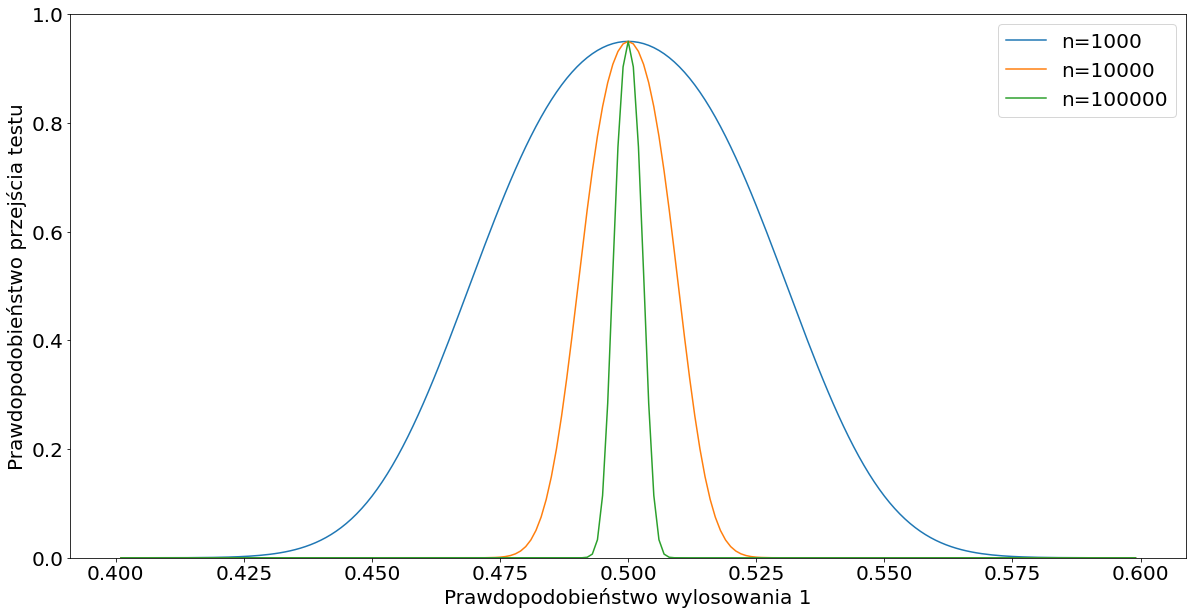
\includegraphics[width=15cm]{chance_of_passing_test_for_n}
    \caption{Porównanie prawdopodobieństwa przejścia testu dla różnych $n$}
    \label{fig:vis_1}
\end{figure}
\begin{figure}[!htp]
    \centering
    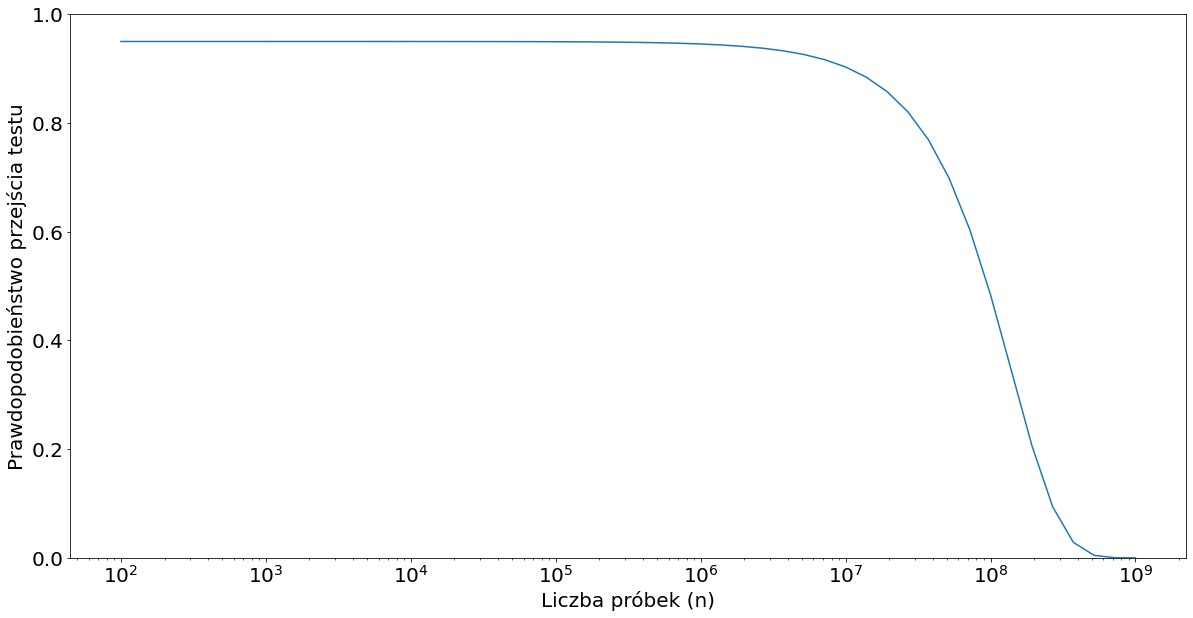
\includegraphics[width=15cm]{probability_of_passing_test_log_scale}
    \caption{Porównanie prawdopodobieństwa przejścia testu dla różnych $n$ (skala logarytmiczna) przy błędzie rozkładu $10^{-3}$}
    \label{fig:vis_2}
\end{figure}
\subsection{Wybranie akceptowalnych rozkładów}
Zakładając prawdziwość tezy o rozkładzie spełniającym prawo Benforda sprawdzimy ile najbardziej znaczących bitów próbki powinniśmy odrzucić. Przyjmijmy za kryterium przejście testu powyżej w 90\% przypadków dla średniej z $10^8$ bitów ($n=10^8$).
\begin{figure}[!htp]
    \centering
    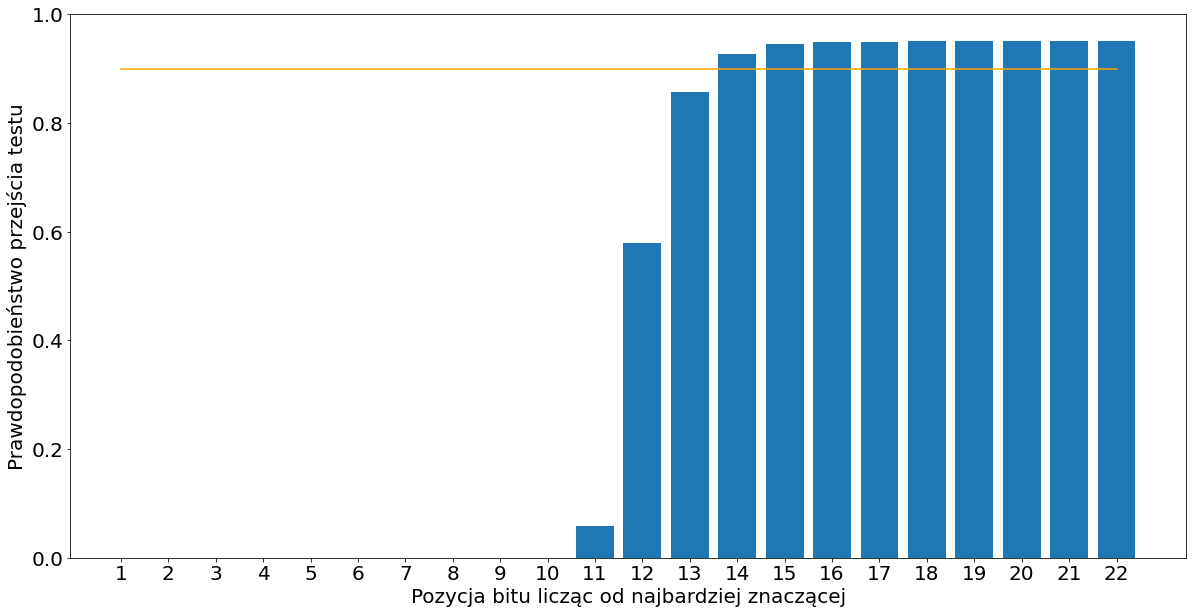
\includegraphics[width=15cm]{probabilty_of_passing_benford}
    \caption{Prawdopodobieństwo przejścia testu statystycznego dla $k$-tego najbardziej znaczącego bitu w próbce spełniającej prawo Benforda (niebieski) oraz próg akceptowalności na poziomie 0.9 (pomarańczowy)}
    \label{fig:probabilty_of_passing_benford}
\end{figure}
Na wykresie \ref{fig:probabilty_of_passing_benford} widzimy, iż bity będące na co najwyżej 14. najbardziej znaczącej pozycji spełniają nasze wymagania. Wcześniejsze niestety będziemy zmuszeni odrzucić ze względu na niekompatybilność rozkładu.
\section{Pseudokod generatora}

{\small
\begin{pseudokod}
\caption{Pseudokod klasy naszego generatora}
\label{alg:gen_code}
\begin{algorithmic}%[1] % uncomment for line numbers
\Class{Generator}
    \State $queue$ : \textsc{SyncQueue<Bit>} \Comment{kolejka synchroniczna bitów}
    \item[]
    \Constructor{$number\_ of\_ threads$ : \textsc{Int}}
        \State $addresses$:\textsc{List<String>} \gets $load()$ \Comment{wczytujemy adresy}
        \For{$i \gets i$ to $number\_of\_threads$}
            \State $thread$ : \textsc{Thread} \gets $Thread$(addresses[i]) \Comment{tworzymy nowy wątek}
            \State $thread$.start() \Comment{uruchamiamy wątek produkujący bity}
        \EndFor
    \EndConstructor
    \item[]
    \Procedure{produce}{$url$ : \textsc{String}}
        \Loop
            \State $time$ : \textsc{Int} \gets $ping$(url) \Comment{pobieramy czas w ns "pinga"}
            \State $bits$ : \textsc{Int} \gets $ceil$($log_2$($time$)) \Comment{obliczamy długość liczby}
            \For{$\_ \gets 14$ to $bits$}
                \State $queue$.push($time$ \textbf{mod} 2) \Comment{dodajemy ostatni bit do kolejki}
                \State $time$ \gets time$ \textbf{div} 2$ \Comment{dzielimy całkowicie przez 2}
            \EndFor
        \EndLoop
    \EndProcedure
    \item[]
    \Function{get}{}
        \State $result$ : \textsc{Int} $\gets 0$
        \For{$\_ \gets 0$ to 63}
            \State $bit$:\textsc{Bit} \gets queue.$pop$() \Comment{pobieramy bit z kolejki}
            \If{$bit$ == 1}
                \State $result$ \gets result $ * 2 + 1$ \Comment{dodajemy 1 na koniec}
            \Else
                \State $result$ \gets result $ * 2$ \Comment{dodajemy 0 na koniec}
            \EndIf
        \EndFor
        \State \Return $result$ \Comment{zwracamy 64-bitową liczbę}
    \EndFunction
\EndClass
\end{algorithmic}
\end{pseudokod}
}
Na podstawie konceptu naszego generatora oraz rozpoznanych potencjalnych problemów możemy przygotować jego pseudokod. Wykorzystamy w nim paradygmat programowania obiektowego, który jest obecnie dostępny w większości najpopularniejszych języków programowania. W pseudokodzie \ref{alg:gen_code} wykorzystamy następujące typy:
\begin{description}
\item[$SyncQueue$] - kolejka synchroniczna. Jest strukturą generyczną, a więc może przechowywać wartości dowolnego określonego typy.  Posiada ona bufor oraz metodę \textbf{$push$} przyjmującą jeden argument, który zostanie dodany do kolejki. W przypadku zapełnienia bufora zatrzymuje wątek do czasu zwolnienia miejsca. Dodatkowo, posiada metodę \textbf{$pop$} która, jeśli bufor nie jest pusty, zdejmuje jeden element z kolejki i go zwraca, a w przypadku pustego bufora zatrzymuje wątek do czasu wprowadzenia do niego danych.
\item[$Thread$] - typ reprezentujący wątek w programie. W konstruktorze przyjmuje funkcję, którą będzie wykonywał po jego uruchomieniu. Wywołanie metody \textbf{$start$} nie zatrzymuje obecnego wątku, a jedynie tworzy nowy. 
\item[$List$] - implementacja listy uporządkowanej.
\item[$Int$] - prosty typ liczbowy 64-bitowy.
\item[$Bit$] - typ liczbowy mogący przyjąć dwie wartości: 0 lub 1.
\item[$String$] - typ przechowujący łańcuch znaków.
\end{description}
Jedynym polem klasy jest $queue$ typu \emph{SyncQueue\textless Bit\textgreater}. Przechowuje ona wygenerowane do tej pory bity, które zostaną wykorzystane w metodzie \emph{get}. Oprócz konstruktora, w którym możemy określić liczbę wykorzystywanych przez nasz generator wątków, mamy dwie metody:
\begin{description}
\item[$produce$] - odpowiada ona za ciągłe pobieranie czasu dostępu do wskazanego w argumencie $url$ adresu, a następnie umieszczanie pozyskanych w ten sposób użytecznych bitów w kolejce $queue$.
\item[$get$] - umożliwia pobieranie liczby losowej z naszego generatora. Bierze ona z kolejki $queue$ 64 bity i tworzy z nich pojedynczą liczbę losową spełniającą założenia tej pracy.
\end{description}

\section{Wybór protokołu do mierzenia czasów połączeń}
Ważnym z punktu widzenia wydajności systemu jest wybór odpowiedniego protokołu sieciowego, który wykorzystamy w naszym generatorze. Nie powinien mieć wpływu na losowość naszych liczb, stąd też możemy koncentrować się na wydajności rozwiązania i wygodzie jego użycia.
\subsection{Przegląd dostępnych rozwiązań}
Przedstawimy tutaj znalezione metody pozyskiwania czasów dostępu do zasobów sieciowych, a mianowicie:
\begin{description}
\item[ping \textit{ICMP} (\textit{Internet Control Message Protocol})] - najbardziej oczywiste podejście do problemu. Jest on obsługiwany przez zdecydowaną większość hostów i powoduje możliwie najmniejsze obciążenie, co pozwala przesłać jednocześnie większą liczbę zapytań z jego wykorzystaniem. Posiada on jednak podstawową wadę - wymaga dodatkowych uprawnień w celu jego wysłania na współczesnych systemach operacyjnych. Oznacza to konieczność uruchamiania programów z tym generatorem z uprawieniami administratora. Ponadto, zupełnie uniemożliwia jego wykorzystanie w niektórych przypadkach, takich jak front-end aplikacji webowych.
\item[\textit{HTTP} (\textit{HyperText Transfer Protocol})] - niezwykle popularny protokół. Wykorzystuje on $TCP$. Z uwagi na to, że wykorzystują go serwisy webowe znalezienie hostów, z którymi można się połączyć nie stanowi żadnego problemu. Ogromną zaletą tego protokołu jest znacząca liczba bibliotek, które go wspierają. Pozwalają one w większości języków pobrać zawartość strony w jednej linijce kodu. Problemem tego podejścia jest natomiast stosunkowo duży rozmiar pakietów, który zależy od wybranego hosta. Dla przykładu kod źródłowy strony \url{http://www.google.com} waży 128 KB, co nie jest relatywnie ogromną wartością, lecz w przypadku konieczności pobrania milionów takich stron mocno obciąża sieć.  
\item[ping \textit{TCP} (\textit{Transmission Control Protocol})] - inne dobre rozwiązanie umożliwiające mierznie czasu potrzebnego na nawiązanie sesji w protokole \emph{TCP}. Naturalnie nie został on zaprojektowany do mierzenia opóźnień, stąd też nie jest tak lekki jak \emph{ICMP}, a więc wywołuje większe obciążenie sieci. Zaletą tego rozwiązania jest brak konieczności posiadania specjalnych uprawnień, przez co możemy go wykorzystać w prawie każdej sytuacji. Wadą jest jednak fakt, iż pingowanie używając tej metody nie jest powszechne. Dlatego też nie zawsze znajdziemy proste w użyciu biblioteki to umożliwiające. Na szczęście, prawie każdy język ma wbudowane wsparcie dla \textit{socketów}. Mając taką bibliotekę wystarczy napisać funkcję nawiązującą połączenie i natychmiast je zrywającą, zmierzyć potrzebny na to czas. Dodatkową wadą jest to, że ciągłe nawiązywanie i zrywanie połączenia nie jest naturalnym zachowaniem w sieci, stąd też po kilku takich próbach, następujących w krótkich odstępach, czas odpowiedzi hosta będzie mocno się wydłużał.
\end{description}
\subsection{Wybór odpowiedniego protokołu}
Jak widzimy, każda z 3 dostępnych opcji niesie z sobą kilka wad, jak i zalet. Na potrzeby tej pracy zastosujemy ostatnie rozwiązanie - tak zwany ping \textit{TCP}. Generator do testów napiszemy w języku Python. Posiada on wsparcie dla tworzenia \textit{socketów}. W przypadku jego implementacji na front-endzie aplikacji webowej, musielibyśmy skorzystać z \textit{web-socketów}. Konieczność nadawania uprawnień administratora dla każdego uruchomienia programu jest w zbyt dużym utrudnieniem dla użytkownika aby zdecydować się na ten wariant z protokołem \textit{ICMP}. Zmiana wybranego protokołu w już zaimplementowanym generatorze nie jest trudna ze względu na jego prostą strukturę. Bez problemu można użyć bibliotek takich jak: \emph{pyping} (dla pingu \textit{ICMP}), \emph{requests} (dla pobierania zawartości stron) oraz \emph{tcping} (dla pinga w oparciu o protokół \textit{TCP}).
\section{Implementacja w języku Python}
Poniżej znajdziemy kod źródłowy \ref{code:source} naszego generatora. Ze względu na jego stosunkowo małą długość pozwolimy sobie omówić go w całości.
\begin{small}
\lstinputlisting[language=Python, caption=Klasa generatora w języku Python, frame=lines, label=code:source, escapechar=#|]{state_of_art.py}
\end{small}
Warto zwrócić uwagę na dwie użyte stałe:
\begin{description}
\item[TIMER\_RESOLUTION\_IN\_NS] - stałą użyta w linijce \ref{line:time_res}. Określa ona rozdzielczość czasu dla funkcji \emph{perf\_counter\_ns}, a więc najmniejsza zmiana, która powoduje zwrócenie innego wyniku. Wpływa ona bezpośrednio na ilość bitów informacji możliwych do uzyskania z pojedynczej próbki.
\item[MOST\_SIGNIFICANT\_BITS\_TO\_REJECT] - stała zastosowana w lilijce \ref{line:bits_reject}. Oznacza ona liczbę najbardziej znaczących bitów z każdej próbki, którą będziemy odrzucać ze względu na występowanie prawa Benforda.
\end{description}
Dodatkowo napisaliśmy funkcje pomocnicze:
\begin{description}
\item[$ping$] -  w linijce \ref{line:ping}. Tworzy ona domyślny \textit{socket}, a następnie łączy się z hostem z argumentu \emph{address} na porcie 80 używanym przez protokół \emph{HTTP}. Po ustanowieniu połączenia go zrywa.
\item[$load\_file$] - w linijce \ref{line:loadfile}. Wczytuje ona kolejne linie z pliku o nazwie pobranej z argumentu \emph{file\_name} i zapisuje je w liście, która jest zwracana na końcu.
\item[$elapsed$] - w linijce \ref{line:elapsed}. Mierzy ona czas potrzebny na wykonanie funkcji przekazanej w argumencie \emph{fn}, a następnie zwraca wynik w jednostce zapewniającej maksymalną ilość informacji o upłyniętym czasie.
\end{description}
Kod zawiera dwie główne klasy:
\begin{description}
    \item[$Pinger$] - którą możemy znaleźć w linijce \ref{line:pinger}. rozszerzającą klasę wątku. Jej głównym zadaniem jest kolejne odpytywanie adresów z argumentu \emph{addresses}, a następne wysyłanie bitów o odpowiednim rozkładzie za pomocą kanału \emph{output}. Dodatkowo w linijce \ref{line:pinger_stop}. znajduje się procedura \emph{stop}, która pozwala zatrzymać wykonywanie wątku.
    \item[$Generator$] - znajduje się w linijce \ref{line:generator}. Jej zadaniem jest generowanie liczb 64-bitowych na podstawie czasów dostępu do zasobów sieciowych. W konstruktorze przyjmuje ona jeden parametr \emph{threads}, który określa ile wątków będzie wykorzystywał generator do pozyskiwania losowych bitów z czasów dostępu do zasobów sieciowych. Dodatkowo konstruktor wczytuje zawartość pliku zawierającego adresy, do których można się połączyć. Funkcja \emph{get}, którą znajdziemy w linijce \ref{line:get}. pobiera bity z kolejki \emph{\_queue}, a następnie tworzy z nich jedną liczbę losową. Klasa zawiera również metodę \emph{stop} w linijce \ref{line:generator_stop}., której zadaniem jest zakończenie pracy generatora oraz wykorzystywanych przez niego wątków. 
\end{description}
\section{Ocena wydajności generatora}
Po zaimplementowaniu generatora możemy dokonać analizy jego wydajności, a więc określić ile losowych bitów będzie w stanie wyprodukować w ciągu sekundy.
\subsection{Ocena wydajności dla pojedynczego wątku}
\sloppy Jak możemy zobaczyć w kodzie w linijce \ref{line:elapsed}. metoda \emph{elapsed} wykorzystuje metodę \emph{time.pref\_counter\_ns}. Według dokumentacji \cite{PythonTimeDoc} dla systemu Windows zapewnia ona rozdzielczość czasu na poziomie 100 nanosekund. Oznacza to, że z każdymi upłyniętymi 100 ns funkcja \emph{time.pref\_counter\_ns} zwróci inny wynik. Dzieląc go przez 100 możemy uzyskać liczbę składającą się z maksymalnej ilości użytecznych bitów. Każdy wątek czeka do czasu otrzymania odpowiedzi z serwera, zatem ilość wykonanych pingów w ciągu sekundy zależy od czasu oczekiwania na odpowiedź. Z drugiej strony im dłuższy czas tym więcej użytecznych bitów otrzymujemy. Zdecydowaliśmy się odrzucać 13 pierwszych bitów ze względu na ich rozkład, a więc próbki poniżej 800 $\mu$s nie niosą żadnej informacji. Na rysunku \ref{fig:generated_bits_in_time} widzimy wydajność pojedynczego wątku dla różnych czasów pinga.
\begin{figure}[!htp]
    \centering
    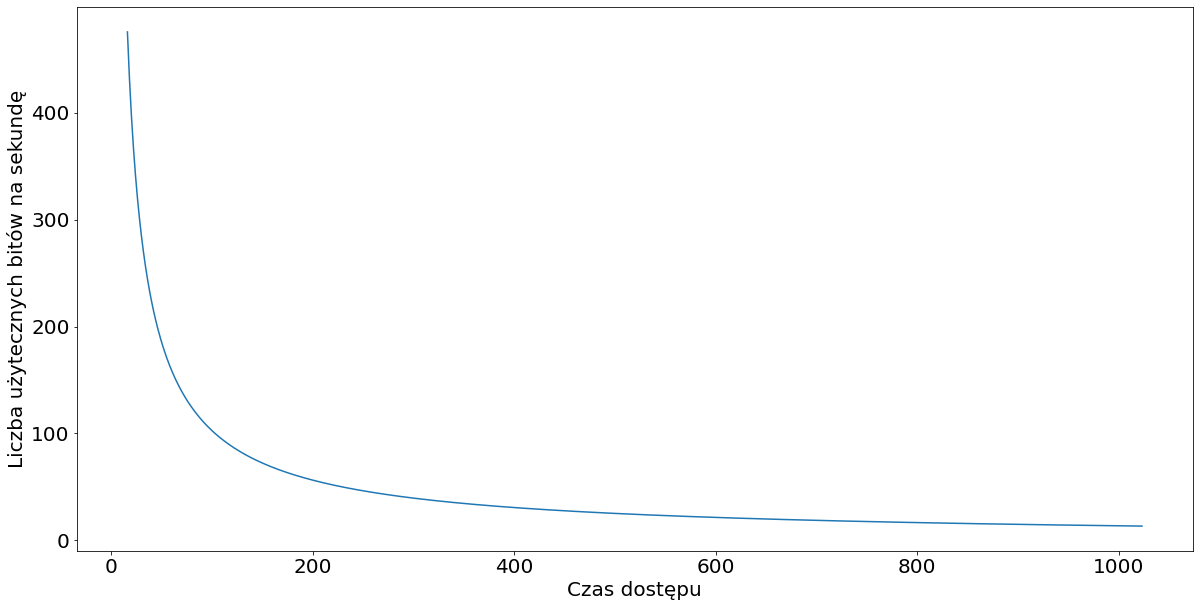
\includegraphics[width=15cm]{generated_bits_in_time}
    \caption{Liczba akceptowalnych bitów uzyskiwanych na jedną milisekundę (oś y), przy stałym czasie pinga w milisekundach (oś x) }
    \label{fig:generated_bits_in_time}
\end{figure}
W praktyce nie udaje się uzyskać czasów lepszych niż 16ms, jeśli chcemy połączyć się do urządzenia spoza naszej sieli lokalnej. W takim przypadku z pojedynczego wątku możemy uzyskać nawet 60 B/s. Jest to relatywnie dobry wynik, choć wypada niezwykle blado w porównaniu z generatorami liczb pseudolosowych. W praktyce jednak średni czas dla pojedynczego pigna w testach wynosił ok. 121 ms. W tym przypadku możemy spodziewać się wydajności rzędu 11 B/s, czyli ok. trzy 64-bitowe liczby losowe na sekundę.  
\subsection{Ograniczenie przez przepustowość sieci}
Aby oszacować jakie obciążenie sieci spowoduje wysłanie jednego pinga \emph{TCP} musimy najpierw zrozumieć jego podstawy. \emph{TCP} jest protokołem połączeniowym, zatem pojedynczy ping wymaga nawiązania połączenia, a następne jego zerwania. 
\begin{figure}[!htp]
    \centering
    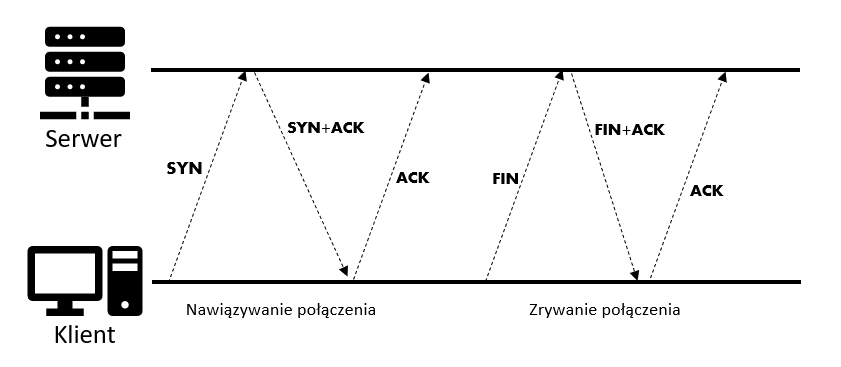
\includegraphics[width=13cm]{tcp_model}
    \caption{Diagram wysyłanych pakietów przy nawiązywaniu i zrywaniu połączenia w protokole TCP}
    \label{fig:tcp_model}
\end{figure}
Jak widzimy na rysunku \ref{fig:tcp_model} ta operacja wymaga wysłania 4 pakietów, przy czym dodatkowo powinniśmy otrzymać 2 pakiety od serwera. Każdy z nich waży od 60 do 80 bajtów. Wykorzystując górne oszacowanie widzimy, że pojedynczy ping wymaga wysłania 320 bajtów oraz pobrania 160 bajtów. Większość dostawców internetu sprzedaje pakiety, których przepustowość wysyłania jest mniejsza od przepustowości pobierania, zatem skupimy się na limicie przepustowości wysyłania. Zakładając, że mamy do dyspozycji łącze o przepustowości wysyłania 1 Mbps, teoretycznie powinniśmy mieć możliwość wykonania 390 pingów na sekundę. Dodatkowym czynnikiem, jaki należy wziąć pod uwagę, jest koszt wykorzystania usługi $DNS$ (\emph{domain name system}). Tłumaczy ona adresy domenowe takie jak \url{www.google.pl} na adresy IP. Jeśli chcemy wykorzystywać adresy w formie domenowej, będziemy umieli do każdego pinga doliczyć ok. 120 bajtów wysłanych oraz 120 bajtów pobranych. Zatem tym samym łączem o przepustowości wysyłania 1 Mbps będziemy teoretycznie mogli wykonać 284 pingów na sekundę.
\subsection{Eksperymentalne wyniki w środowisku testowym}
Znając teoretyczne ograniczenia wydajności naszego generatora warto sprawdzić jak w stosunku do teoretycznych ograniczeń wypada jego wydajność w środowisku testowym. Testy zostały wykonane na prywatnym komputerze w niedzielę o godzinie 18:00. Według serwisu \url{https://www.speedtest.net} wykorzystane połączenie miało 83.75 Mbps przepustowości pobierania oraz 24.29 Mbps przepustowości wysyłania. Zbadaliśmy liczbę pingów na sekundę przy różnej liczbie jednoczesnych pingów. 
\begin{figure}[!htp]
    \centering
    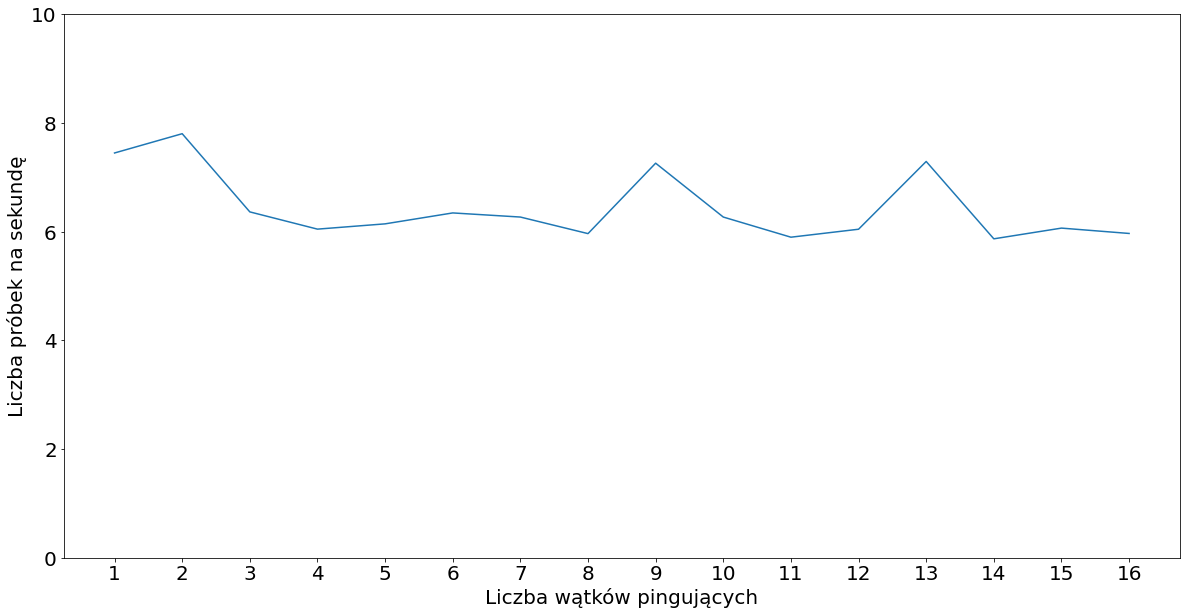
\includegraphics[width=15cm]{performance}
    \caption{Wykres zestawiający liczbę jednoczesnych wątków (oś $x$) z liczbą pingów na sekundę (oś $y$)}
    \label{fig:performance}
\end{figure}
Jak możemy zobaczyć na rysunku \ref{fig:performance}, nie została wykazana żadna istotna korelacja między liczbą wątków a ogólną wydajnością generatora. Spore wahania w wydajności dla różnej liczby wątków zostały prawdopodobnie spowodowane różnicami w obciążeniu sieci w momencie testu. Brak zwiększonej wydajności w przypadku generatora z większą liczbą wątków jest najprawdopodobniej spowodowany limitem ilości przesyłanych pakietów przez lokalny router lub dostawcę internetu. Dalsze badania są wymagane w celu jednoznacznego ustalenia przyczyny problemów z straconymi pakietami w przypadku testów z dużą liczbą jednoczesnych pingów.